\documentclass[titlepage]{report}

\usepackage[margin=1in]{geometry}
\usepackage{fancyhdr}
\usepackage{csquotes}
\usepackage{marginnote}
\usepackage{scrextend}
\usepackage[bottom]{footmisc}
\usepackage{enumitem}
\usepackage{xr}
\usepackage{amsmath,amssymb,amsthm}
\usepackage{mathtools,physics}
\usepackage{tikz,graphicx,subcaption}
\usepackage[hidelinks]{hyperref}

\fancypagestyle{plain}{
    \fancyhead{}
    \renewcommand{\headrulewidth}{0pt}
}
\fancypagestyle{main}{
    \fancyhf{}
    \fancyhead[L]{\leftmark}
    \fancyhead[R]{MATH 16110}
    \fancyfoot[R]{Labalme \thepage}
}

\MakeOuterQuote{"}

\reversemarginpar

\deffootnotemark{\textsuperscript{\textup{[}\thefootnotemark\textup{]}}}
\deffootnote[2.1em]{0em}{0em}{\textsuperscript{\thefootnote}}

\setitemize[3]{label={\scriptsize$\blacksquare$}}

\DeclareMathOperator{\ext}{ext}

\newtheorem{theorem}{Theorem}[chapter]
\newtheorem{proposition}[theorem]{Proposition}
\newtheorem{lemma}[theorem]{Lemma}
\newtheorem{corollary}[theorem]{Corollary}
\newtheorem{axiom}{Axiom}
\newtheorem*{axioms}{Axioms}
\newtheorem*{theorem*}{Theorem}
\newtheorem*{lemma*}{Lemma}
\newtheorem{lemmaM}{Lemma}
\newtheorem{corollaryM}{Corollary}
\theoremstyle{definition}
\newtheorem{definition}[theorem]{Definition}
\newtheorem{exercise}[theorem]{Exercise}
\newtheorem{remark}[theorem]{Remark}
\newtheorem*{definition*}{Definition}
\newtheorem{exerciseM}{Exercise}

\usetikzlibrary{positioning,shapes,decorations.pathreplacing,calc}

\renewcommand{\chaptername}{Script}

\newcommand{\N}{\mathbb{N}}
\newcommand{\Z}{\mathbb{Z}}
\newcommand{\mA}{\mathcal{A}}
\newcommand{\Q}{\mathbb{Q}}
\newcommand{\eqclass}[2]{\left[ \frac{#1}{#2} \right]}
\newcommand{\plusQ}{+_\Q}
\newcommand{\cdotQ}{\cdot_\Q}
\newcommand{\lQ}{<_\Q}

\usepackage{subfiles}

\title{MATH 16110 (Honors Calculus I IBL) Notes}
\author{Steven Labalme}

\begin{document}




\maketitle



\pagenumbering{roman}
\tableofcontents
\listoffigures
\newpage



\pagenumbering{arabic}
\pagestyle{main}
\subfile{NotesOnProofs/notesonproofs.tex}



\setcounter{secnumdepth}{3}
\subfile{Script0/script0.tex}


\section{Discussion}
\begin{itemize}
    \item \marginnote{10/8:}How much of the proof of Additional Exercise \ref{axr:0.7} proof could be left out as unnecessary verbage?
\end{itemize}



\subfile{Script1/script1.tex}


\section{Discussion}
\begin{itemize}
    \item \marginnote{10/1:}Always make sure you use all given assumptions.
    \item We are allowed to assume that $x\in\{A:Q\}$ tells us that $x\in A$ and $Q$ is true? --- yes.
    \item We can let $x$ be an arbitrary element of a set and deduce stuff like in Tao.
    \item When we're writing proofs (consider Theorem \ref{trm:1.12}), do we do not have to show the definition of $A\cap B$? --- we can just say "by Definition \ref{dfn:1.6}, $y\notin A\cap B$ implies that $y\notin a$ or $y\notin b$."
    \begin{figure}[h!]
        \centering
        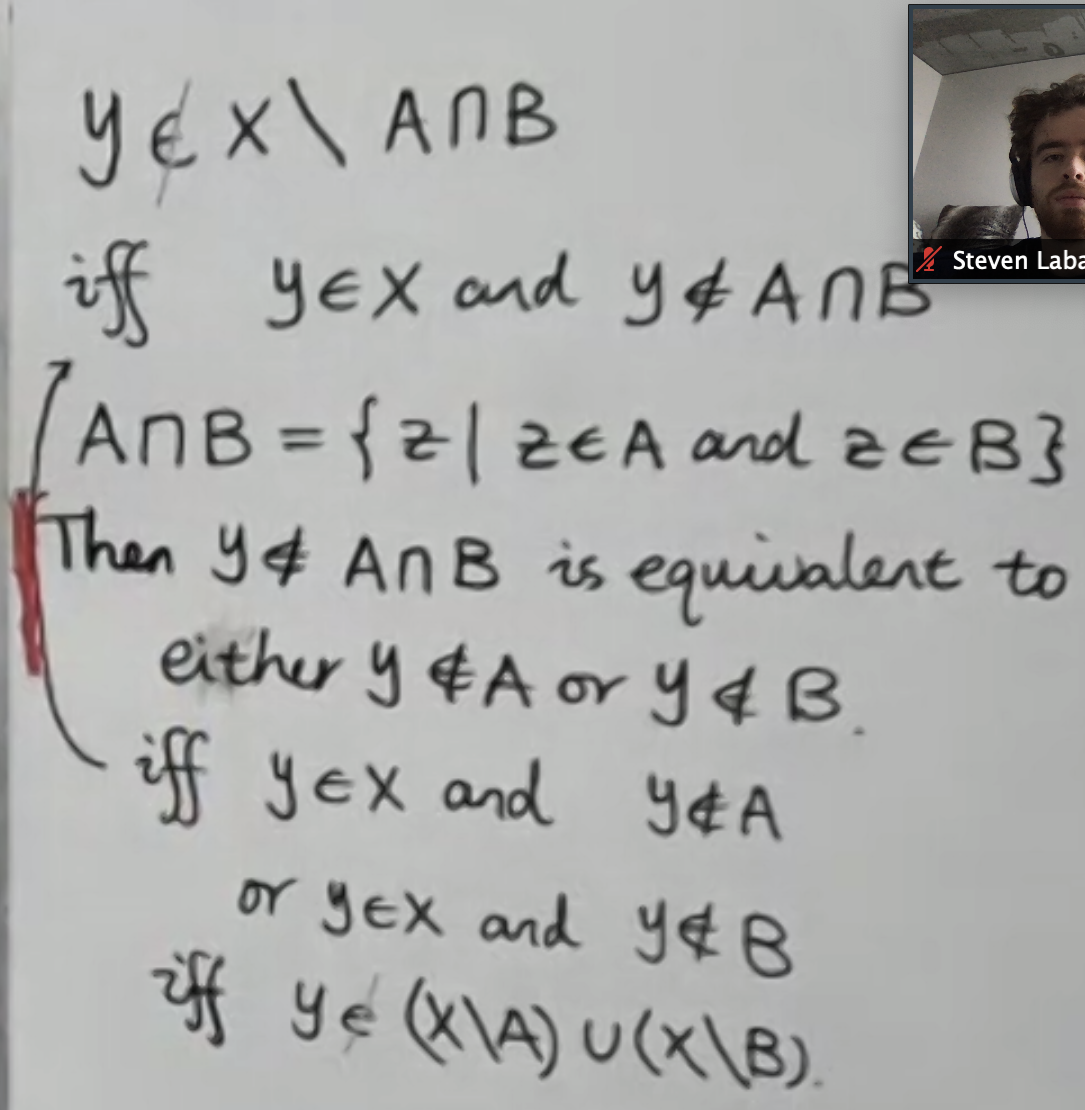
\includegraphics[width=0.3\linewidth]{ExtFiles/SampleTrm1-12Proof.png}
        \caption{Sample exam-ready proof of Theorem \ref{trm:1.12}.}
        \label{fig:sampleTrm1-12Proof}
    \end{figure}
    \item What he wrote for the beginning of the proof of Theorem \ref{trm:1.12} (see Figure \ref{fig:sampleTrm1-12Proof}) is acceptable on an exam; in our exams, it will be the same as when presenting to class (we do not need complete sentences).
    \item Can we say "A similar argument works in reverse?"
    \item \marginnote{10/6:}Vacuous truths were introduced.
    \item If you had to prove your answers to Additional Exercise \ref{axr:1.1}, you would write out the elements of the first set, and rewrite the elements with each additional constraint.
    \begin{itemize}
        \item For example, $(\{n\in\Z\mid n\text{ is divisible by }2\}\cap\N)\cup\{-5\}=(\{\cdots,-4,-2,0,2,4,\cdots\}\cap\{1,2,3,\cdots\})\cup\{-5\}=\{2,4,6,\cdots\}\cup\{-5\}$.
    \end{itemize}
    \item In this class, $0\notin\N$, but $0\in\N_0$.
    \item For Exercise \ref{exr:1.21}, we can refer to Theorem 7 in "Notes on proofs" to demonstrate that $\sqrt{2}\notin\N$.
    \item When presenting, write on the board more like I would in a journal.
    \item Ask about my contradiction proofs for 1.21-1.23!
    \item \marginnote{10/8:}! means "unique."
    \item $\because$ means "since."
    \item \marginnote{10/13:}What are your office hours? Mondays 4-6 PM.
    \item Do I need to submit the LaTeX assignment to you? Email it to him!
    \item Edit this document to reflect switch to section 22!
    \item Script \ref{sct:2} sign up sheet is on Canvas (sign up within 24 hours)!
    \item \marginnote{10/15:}Informal explanation of $10^a+10^b=10^c+10^d$ is ok.
\end{itemize}



\subfile{Script2/script2.tex}


\section{Discussion}
\begin{itemize}
    \item \marginnote{10/15:}Divisibility (see Exercise \ref{exr:2.2d}) is defined in terms of multiplication in Script \ref{sct:0}. Thus, I should use $y-x=5a$ for some $a\in X$ instead of $\frac{y-x}{5}\in X$.
    \item At the end of the proof of Exercise \ref{exr:2.2e}, do casework on $c$ ($c=0$ and $c\neq 0$) to stymie accusations of dividing by 0.
    \item Exercise \ref{exr:2.6}:
    \begin{itemize}
        \item Note that we cannot always pick an arbitrary element of a set (e.g., if a set is empty). However, by definition, $\eqclass{a}{b}$ is nonempty, so we \emph{can} pick an arbitrary element in it.
        \begin{itemize}
            \item Additionally, note that we are probably fine not getting into this technicality because performing any operation on a hypothetical $x\in\emptyset$ invokes vacuous (i.e., weird but still sound) logic.
        \end{itemize}
        \item Let $(x_1,x_2)$ be an arbitrary element of the left set. It is therefore related to $(a,b)$. By set equality, it is an element of the right set. Thus, $(x_1,x_2)\sim(a',b')$. Use symmetry/transitivity to show $(a,b)\sim(a',b')$.
    \end{itemize}
    \item Rewrite Theorem \ref{trm:2.8} as a direct proof.
    \item Journal format: Turning in what I have in this document is fine.
    \item \marginnote{10/20:}Edit Exercise \ref{exr:2.2d} to use Additional Exercise \ref{axr:0.8-i}!
    \item Do we have to prove injectivity for $h$ in Theorem \ref{trm:2.11}? (Injectivity implies bijectivity by Exercise \ref{exr:1.38}.)
    \begin{itemize}
        \item Yes, we still have to prove injectivity here.
    \end{itemize}
    \item Technically, you have to prove that $\N$ is countable, but Cartee won't be looking for it --- you won't have to prove it for credit.
    \item You can also use a lemma that a surjection $f:A\to B$ where $A$ is countable and $B$ is infinite implies that $B$ is countable.
    \item $\gcd(a,b)$ is defined as the largest natural number by which $a$ and $b$ are both divisible.
    \item We want to pick the pair in the equivalence class that has the lowest possible, positive denominator. Think about it in terms of the well-ordering principle. You get a huge set of pairs, look at the subset with positive denominators, then look at just the denominators. You would have to explain why one denominator corresponds to one ordered pair.
    \item Use $f(\eqclass{a}{b})=(a',b')$ to denote that $a\neq a'$ and $b\neq b'$ in every case although the numbers are related.
    \item Two things in the same equivalence class go to the same place, whereas two things in different equivalent classes go to different places.
    \item We're restricting the range with the well-ordering principle, not the domain.
    \item \marginnote{11/10:}The axiom of choice is necessary for my proof of Theorem \ref{trm:2.11} to work. See the edits to the proof of Lemma (a).
    \begin{itemize}
        \item However, a proof using the well-ordering principle (which works as a selector function) would be better than invoking the axiom of choice in the eyes of some mathematicians.
    \end{itemize}
\end{itemize}



\subfile{Script3/script3.tex}


\section{Discussion}
\begin{itemize}
    \item \marginnote{10/20:}Show that $|\{x\}|=1$? Perhaps in a lemma by defining a singleton set. Also make sure that it's clear that $A\cap\{x\}=\emptyset$ to use Theorem \ref{trm:1.34b}.
    \begin{itemize}
        \item Using $B=A\setminus\{x\}$ might help in identifying that $x$ exists, and would help in $B\cap\{x\}=\emptyset$. Thus, $|\{x\}|+|B|=|A|$, it follows by subtraction that $|B|=n$. Potentially as a lemma so I can use it in Theorem \ref{trm:3.5}, too?
    \end{itemize}
    \item Consider case in Theorem \ref{trm:3.5} that $A$ is empty.
    \item What is a limit point?
    \begin{itemize}
        \item A point $p$ would be a limit point of a set $A$ if there's a point $p$ to which the elements of $A$ converge. So on an open interval, the limit points would be the two "end points" and every point therein.
        \item No limit points on the integers. Yes on the rationals and reals.
    \end{itemize}
    \item \marginnote{10/22:}For Exercises \ref{exr:3.9a} and \ref{exr:3.9c}, it is necessary to show that at least one of the three trichotomy statements holds.
    \item \marginnote{10/27:}Do we have to show the explicit proof of both cases in the second part of Lemma \ref{lem:3.16}, or can we just say, "the proof is symmetric?"
    \item In Theorem \ref{trm:3.18}, you can define two functions $\min:C\times C\to C$ and $\max:C\times C\to C$, where $C$ is the continuum in which the two regions exist, by
    \begin{align*}
        \min(i,j) &=
        \begin{cases}
            i & i\leq j\\
            j & i>j
        \end{cases}\\
        \max(i,j) &=
        \begin{cases}
            i & i\geq j\\
            j & i<j
        \end{cases}
    \end{align*}
    for any $i,j\in C$.
    \begin{itemize}
        \item This allows you to define $m=\max(a,c)$ and $n=\min(b,d)$. It can then be proven that $m<n$ in every case, that $\underline{ab}\cap\underline{cd}=\underline{mn}$, and that $x\in\underline{mn}$.
    \end{itemize}
    \item Note that Lemmas \ref{lem:3.16} and \ref{lem:3.17} cannot be used to prove Theorem \ref{trm:3.18} --- the ordering in the script is just misleading (these lemmas will only be needed later).
    \item You don't need to treat all four cases in Theorem \ref{trm:3.18}; rather, just two and then the others are covered by WLOG.
    \begin{itemize}
        \item $
            a>c\wedge b\leq d \xRightarrow{\text{rename}} c>a\wedge d\leq b
            \Rightarrow (a\leq c\wedge b>d)\vee(a\leq c\wedge b=d)
        $, where both of the latter two cases are covered by one of the original cases.
    \end{itemize}
    \item What is the base case in Corollary \ref{cly:3.19}? Although the question does not explicitly state that we can, we should use $n_0=2$ and the form of induction in Additional Exercise \ref{axr:0.2a}.
    \item In Corollary \ref{cly:3.19}, use summation notation, e.g., $\bigcap_{i=1}^k R_i$!
    \item Do the forward implication of Theorem \ref{trm:3.20} by contrapositive.
    \item Use Theorem \ref{trm:3.18} to justify $R_1\cap R_2=R$ in the proof of Theorem \ref{trm:3.20}.
    \item Do I have to prove the two set theory things I use in my proof of Theorem \ref{trm:3.20}?
    \item \marginnote{10/29:}There are several possible proofs for Theorem \ref{trm:3.24}. While induction is correct, the simplest is as follows.
    \begin{itemize}
        \item Label the elements $a_1,\dots,a_n$ (Theorem \ref{trm:3.5}).
        \item Partition $A$ into $n$ singleton sets (such a partitioning may be verified via induction).
        \item If $p\in LP(A)$, then $p\in\{a_k\}$ (Corollary \ref{3.21}), but we cannot have $p\in\{a_k\}$ by Corollary \ref{cly:3.23}.
    \end{itemize}
    \item Alternate proof of Corollary \ref{cly:3.25}:
    \begin{itemize}
        \item Finite $A\subset C \xRightarrow{\text{Theorem \ref{trm:3.24}}} LP(A)=\emptyset \Longrightarrow p\notin LP(A)\ \forall\ x\in C$.
        \item $\xRightarrow{\text{Definition \ref{dfn:3.13}}} \exists\ R:p\in R\vee R\cap(A\setminus\{p\})=\emptyset$.
        \begin{itemize}
            \item $\Rightarrow (R\cap A)\setminus\{p\}=\emptyset$.
            \item $\xRightarrow{\text{Definition \ref{dfn:1.11}}}\nexists\ y\in R\cap A:y\notin\{p\}$, i.e., $\forall\ y\in R\cap A$, $y\in\{p\}$.
            \item $\xRightarrow{\text{Definition \ref{dfn:1.3}}}R\cap A\subset\{p\}$.
        \end{itemize}
        \item $p\in A\vee p\in R \xRightarrow{\text{Definition \ref{dfn:1.6}}}p\in A\cap R$
        \begin{itemize}
            \item $\xRightarrow{\text{Definition \ref{dfn:1.3}}}\{p\}\subset A\cap R$
        \end{itemize}
        \item $R\cap A\subset\{p\}\vee\{p\}\subset R\cap A \xRightarrow{\text{Theorem \ref{trm:1.7}}} R\cap A=\{x\}$.
    \end{itemize}
    \item The method used in Theorem \ref{trm:3.26}, is the best, but it could likely be done by inducting to prove that $|R\cap A|$ cannot equal any natural number (to find contradictions for all $n\in\N$).
    \begin{itemize}
        \item If there was a finite number of elements in $R$, they could be ordered as in Theorem \ref{trm:3.5}. If $a_i<p<a_{i+1}$, then $\underline{a_ia_{i+1}}$ would be an empty $p$-containing region.
    \end{itemize}
    \item The set of all grammatically correct English sentences is a continuum: Define $f:\text{alphabet}\to\Z$ by
    \begin{equation*}
        f(\alpha) =
        \begin{cases}
            1 & \alpha=a\\
            -1 & \alpha=y\\
            0 & \alpha\neq a\vee\alpha\neq y
        \end{cases}
    \end{equation*}
    Add "which is yellow" to sentences to prove that there is no first point. Add "which is amusing" to sentences to prove that there is no last point. These modifiers can be added on indefinitely, and although you generally wouldn't, it's all grammatically correct.
    \item $\Z$ and $\Q$ both satisfy all of the axioms, and there is a bijection between them, yet one is dense and the other isn't. So\dots
    \item \marginnote{11/3:}First attempt at formalizing "the same": Two continuua are the same iff they are in bijective correspondence.
    \begin{itemize}
        \item Flaws: A bijection between $\Z$ and $\Q$ is a necessary condition for them being "the same," but it's not a sufficient condition.
        \item $\Q$ is "dense" whereas $\Z$ is not.
        \item Thus, we must include a proto-definition of density (or somehow assert that the bijection "preserves the ordering").
    \end{itemize}
    \item Second attempt at formalizing "the same": Two continuua are the same iff there exists a bijection $f:A\to B$ such that $f(a)<f(b)$ iff $a<b$.
    \begin{itemize}
        \item Alternate formulation for density: Let $C$ be a continnuum. $C$ is dense iff for all regions $R\subset C$, $LP(R)\neq\emptyset$.
        \item Flaws: If there are two continua $A,B$ that meet the condition "there exists a bijection $f:A\to B$ such that $f(a)<f(b)$ iff $a<b$," then the latter condition implies that they are either both dense or both not dense. Basically, dense/non-dense is a dichotomy; we need a categorization method that is a \emph{trichotomy} (as per Cartee), perhaps one that includes dense, "non-dense," and some third category.
    \end{itemize}
    \item Proof that the condition implies that $A$ and $B$ are either both dense or both not dense:
    \begin{itemize}
        \item Let $a,b$ be arbitrary elements of $A$ such that $a<b$.
        \item If $A$ is dense, then there exists an element $c\in A$ such that $a<c<b$. Now if $B$ is not dense, then we cannot guarantee that there exists an element $d\in B$ such that $f(a)<d<f(b)$. Thus, we cannot guarantee that $f(a)<f(c)<f(b)$. So $B$ must be dense.
        \item If $A$ is not dense, the proof is similar to the above argument in reverse.
    \end{itemize}
    \item Final conclusion: Constraints for two continua $A,B$ to be "the same":
    \begin{enumerate}
        \item There must exist a bijection $f:A\to B$.
        \item $A$ and $B$ must be of the same density category (both dense, both semi-dense, or both buoyant).
    \end{enumerate}
    \item \textbf{Dense} (continuum): A continuum $C$ such that for all regions $R\subset C$, $LP(R)\neq\emptyset$.
    \item \textbf{Semi-dense} (continuum): A continuum $C$ such that for some region $R\subset C$, $LP(R)\neq\emptyset$, and for some region $S\subset C$, $LP(S)=\emptyset$.
    \item \textbf{Buoyant} (continuum): A continuum $C$ that is neither dense nor semi-dense. Equivalently, for all regions $R\subset C$, $LP(R)=\emptyset$.
    \item Note that there are multiple semi-dense continuua that could be argued are different but are the same under this definition (say if there were only one dense "region" versus two dense "regions"). We might want to split into \textbf{hemi-dense} and other categories, but for now, we're going with this.
    \item We conclude by considering three continua, one of each kind, as the concrete realizations requested by Exercise \ref{exr:3.27}: $\Z$ (buoyant), $\Q$ (dense), and $\Q\setminus\underline{01}$ (semi-dense).
    \begin{figure}[h!]
        \centering
        \begin{subfigure}[b]{0.32\linewidth}
            \centering
            \begin{tikzpicture}
                \footnotesize
                \draw [<->] (-2,0) -- node[above=2mm]{$\Q$} node[below=1mm]{\textcolor{white}{0}} (2,0);
            \end{tikzpicture}
            \caption{Dense set.}
            \label{fig:denseSemiBuoyanta}
        \end{subfigure}
        \begin{subfigure}[b]{0.33\linewidth}
            \centering
            \begin{tikzpicture}
                \footnotesize
                \draw [<-|] (-2,0) -- (0,0) node[above=2mm]{$\Q\setminus\underline{01}$} node[below=1mm]{0};
                \draw [|->] (1,0) node[below=1mm]{1} -- (2,0);
            \end{tikzpicture}
            \caption{Semi-dense set.}
            \label{fig:denseSemiBuoyantb}
        \end{subfigure}
        \begin{subfigure}[b]{0.32\linewidth}
            \centering
            \begin{tikzpicture}
                \footnotesize
                \foreach \x in {-1,0,1} {
                    \fill (\x,0) circle (1pt) node[below=1mm]{$\x$};
                }
                \foreach \x in {-2,2} {
                    \node at (\x,0) {$\cdots$};
                }

                \node [above=2mm] {$\Z$};
            \end{tikzpicture}
            \caption{Buoyant set.}
            \label{fig:denseSemiBuoyantc}
        \end{subfigure}
        \caption{A dense, semi-dense, and buoyant number line.}
        \label{fig:denseSemiBuoyant}
    \end{figure}
    \begin{itemize}
        \item A pictoral representation is given above in Figure \ref{fig:denseSemiBuoyant} for each of these sets.
    \end{itemize}
    \item Additional problem: If there exists \emph{a} bijection $f:\Z\to\Q$ (which there is), shouldn't there be one that preserves ordering?
    \begin{itemize}
        \item For one, $f(1)$ cannot be mapped to the smallest, positive, nonzero element of $\Q$, since no such object exists.
        \item Another thing is that since $\Q$ is dense, there exists a $p\in Q$ such that $f(1)<p<f(2)$. But there does not exist any integer between 1 and 2.
        \item And yet \emph{an} element of $\Z$ does map to every element of $\Q$, so can't we "flip" which object maps to which other object? So if $f(2)=\frac{1}{2}$ and $f(z)=\frac{1}{4}$, then can't we let $f(2)=\frac{1}{4}$ and $f(z)=\frac{1}{2}$, and keep "flipping" indefinitely? But then, would we ever actually reach a "limit bijection" with the desired quality? It would simultaneously seem that we would have to and that we never could.
        \item Basically, what the issue boils down to is a potential problem with the ZFC-axioms of set theory and the objects we've defined since. All of these results follow directly from what we assume, but there is the possibility that the base assumptions are wrong. If I can assemble my disparate ideas into a formal paradox (\`{a} la Russell's Paradox with respect to na\"{i}ve set theory), then I would be able to challenge this idea, but until then, I'll let it go.
    \end{itemize}
\end{itemize}



\subfile{Script4/script4.tex}


\section{Discussion}
\begin{itemize}
    \item \marginnote{11/3:}Emily Wilson's more lyrical translation of \emph{The Odyssey}.
    \item \marginnote{11/5:}In Theorem \ref{trm:4.6}, is there a simpler way to prove the lemma?
    \begin{itemize}
        \item Direct approach: $R\cap(LP(X)\setminus\{p\})\neq\emptyset$ implies $R$ contains at least one other limit point of $LP(X)$ besides $p$. Let $m$ be this point. Then $R\cap(X\setminus\{m\})\neq\emptyset$. Therefore, $R\cap X$ is infinite. So $R\cap(X\setminus\{p\})\neq\emptyset$ (it will just be "slightly less infinite"). Therefore, $p\in LP(X)$.
    \end{itemize}
    \item Alternate proof (Theorem \ref{trm:4.10} part 2): Now suppose that $G$ is open. Then by Definition \ref{dfn:4.8}, $C\setminus G$ is closed. Let $x$ be an arbitrary element of $G$. We wish to prove that there exists a region $R$ with $x\in R$ such that $R\cap(C\setminus G)=\emptyset$, i.e., $R\cap((C\setminus G)\setminus\{x\})=\emptyset$, i.e., $x\notin LP(C\setminus G)$. Since $C\setminus G$ is closed, $C\setminus G=(C\setminus G)\cup LP(C\setminus G)$ by Definition \ref{dfn:4.1}. Thus, for all $a\in G$, $a\notin C\setminus G$, i.e., $a\notin LP(C\setminus G)$ by the closure of $C\setminus G$. Additionally, we necessarily have that $a\in R$ where $R$ is some region. Thus, $R\cap((C\setminus G)\setminus\{a\})=\emptyset$, i.e., for all $r\in R$, $r\notin C\setminus G$. Thus, $R\subset C\setminus(C\setminus G)=G$.
    \item Alternate proof (Corollary \ref{cly:4.11}): First, address "every $C\setminus R$ is closed." We must show that $LP(C\setminus R)\subset C\setminus R$. If $p\in LP(C\setminus R)$, then by Definition \ref{dfn:3.13}, $S\cap((C\setminus R)\setminus\{p\})\neq\emptyset$ for all $S\subset C$ such that $p\in S$. Now suppose for the sake of contradiction that $p\notin C\setminus R$. Then $S\cap(C\setminus R)\neq\emptyset$ for all $S\subset C$ with $p\in S$. But since $p\in R$, if we let $S=R$, then $R\cap(C\setminus R)\neq\emptyset$, a contradiction. Thus, $p\in C\setminus R$, so $C\setminus R$ is closed for all regions $R\subset C$.\par
    We have by the first part that $C\setminus R$ is closed for all $R\subset C$. Thus, $R$ is open.
    \item Shiv approached Theorem \ref{trm:4.14} inductively and then considered the infinite case. This is far overcomplicated and likely incorrect, though.
    \item Definitions can be treated as if and only if. More accurately, a definition assigns a term to a certain characteristic in a way similar to if and only if but not identical.
    \item \marginnote{11/10:}How much of a write up do we need for Exercise \ref{exr:4.15}, i.e., fully rigorous, semi-rigorous is ok, somewhere in between?
    \begin{itemize}
        \item Yes, go rigorous all the way.
    \end{itemize}
    \textbf{Axiom of choice}: A Cartesian product of nonempty sets is, itself, nonempty.
    \begin{itemize}
        \item If you have finitely many bins, then for each bin, you can pick one thing out of each bin.
        \item If you have infinitely many bins, then you need the Axiom of choice to pick one thing out of each bin.
        \begin{itemize}
            \item We have nonempty bins, we take their Cartesian product, which is equivalent to picking out an element from each bin and assembling them into a set.
            \item You need a selection function, or assume the axiom of choice.
        \end{itemize}
        \item You don't need the axiom of choice if you know that there is a consistent way of picking something out from any single set.
        \begin{itemize}
            \item Infinitely many pairs of shoes? You can always pick the left shoe.
            \item Infinitely many pairs of socks (which are indistinguishable)? You need the axiom of choice.
        \end{itemize}
        \item Issue first came up in defining $f:\Q\to\Z\times\Z$. We wanted to send $\eqclass{a}{b}$ to a consistent object $(a_1,b_1)\in\Z\times\Z$. With the well-ordering principle, we had a consistent way of picking out an element of $\eqclass{a}{b}$ (the one with the smallest positive nonzero denominator).
    \end{itemize}
    \item So with respect to Theorem \ref{trm:4.14}, we need the axiom of choice.
    \begin{itemize}
        \item Wrong: we cannot iteratively apply Theorem \ref{trm:4.10} to each element $x\in G$ if $G$ is uncountably infinite. To be able to pick out a region for every $x$ "at the same time," we need the axiom of choice. We're taking issue with the creation of the set $\bigcup_{x\in G}R_x$, not actually proving that $\bigcup_{x\in G}R_x=G$, which can be well done for "one arbitrary element."
        \item Wrong: in the proof, say, "...Thus, we can create the set $\mathcal{R}=\{R_x\mid x\in G\}$ [by the axiom of choice] and define its union..."
        \item Right: We use the axiom of choice to pick 1 $R_x$ out of the set of all possible $R_x$ (we know that at least one exists by Theorem \ref{trm:4.10}, but there could be [and certainly in some cases are] infinitely many $R_x$ containing $x$ that are subsets of $G$). It is the act of choosing that necessitates the axiom of choice.
    \end{itemize}
    \item Alternate proof of Theorem \ref{trm:4.14} w/o the axiom of choice:
    \begin{itemize}
        \item Consider the set $\bigcup_{R\subset G}R$, which is the union of all regions $R$ such that $R\subset G$. We prove that $\bigcup_{R\subset G}R=G$. Let $x\in\bigcup_{R\subset G}R$. Then $x\in R$ for some $R\subset G$. It follows that $x\in G$. Now let $x\in G$. Then by Theorem \ref{trm:4.10}, there exists an $R\subset G$ such that $x\in R$. As a region that is a subset of $G$, $R$ is one of the sets in $\bigcup_{R\subset G}R$. Thus, $x\in\bigcup_{R\subset G}R$.
    \end{itemize}
    \item In Exercise \ref{exr:4.15}, show that the region containing 2 is not a subset of $\underline{12}\cup\{2\}$ and then invoke Theorem \ref{trm:4.10} to prove that it's not open. To prove that it's closed, still use my argument.
    \item \marginnote{11/12:}Revisiting the axiom of choice:
    \begin{itemize}
        \item When we have an infinite collection of sets, we either need a selector function that takes in any of the sets and evaluates to one element of that set OR the axiom of choice to pick out one element from every set in this collection.
    \end{itemize}
    \item \marginnote{11/17:}In the proof of Exercise \ref{exr:4.23}, do we have to first show that $C\setminus\{a\}$ is a continuum? And if so, how rigorously?
    \begin{itemize}
        \item Probably not.
    \end{itemize}
    \item What about rigor in Exercise \ref{exr:4.24}?
    \begin{itemize}
        \item Needs to be done rigorously, but we did not figure it out today.
    \end{itemize}
    \item You can use the interval notation $(a,b)$ if you want, as long as it's clear from context what you mean.
    \item \marginnote{11/19:}Proving set equality is an example of a \textbf{bidirectional inclusion proof}.
    \item In Exercise \ref{exr:4.24}, we make use of the continued fraction approximation of $\sqrt{2}$, namely that
    \begin{equation*}
        \sqrt{2} = 2-\frac{2}{2+\sqrt{2}}
    \end{equation*}
    \item The important conclusion from Exercise \ref{exr:4.24} is that while $\Q$ exhibits \textbf{betweenness} (what we earlier called density), it still has holes.
    \item \marginnote{12/3:}Problems with Exercise \ref{exr:4.23}.
    \begin{itemize}
        \item The set $\{x\in C\mid x<a\}$ is open in $C$, not open in $C\setminus\{a\}$.
        \item More specifically, Corollary \ref{cly:4.13} requires that $a\in C$, but $a\notin C\setminus\{a\}$.
        \item Use Theorem \ref{trm:4.10} to show that $\{x\in C\mid x<a\}$ and the other one are open.
        \begin{itemize}
            \item With Theorem \ref{trm:5.2}, we can find a point $c$ such that $x<c<a$.
            \item Then we can find a point $b<x$. Thus, $x\in\underline{bc}$ and $\underline{bc}\subset\{x\in C\mid x<a\}$.
        \end{itemize}
        \item This is a good solution; it's just silly that Exercise \ref{exr:4.23} comes before Theorem \ref{trm:5.2} in the Script chronology.
    \end{itemize}
\end{itemize}



\subfile{Script5/script5.tex}


\section{Discussion}
\begin{itemize}
    \item \marginnote{11/19:}Potentially I can suppose that $A$ is nonempty straightaway to avoid considering the case that $A=\emptyset$ in Theorem \ref{trm:5.1}.
    \item Don't switch to $\leq$ and $\geq$ in Theorem \ref{trm:5.2}! Just use $C=(-\infty,y)\cup(x,+\infty)$, two provably open, disjoint, nonempty sets.
    \item Theorem \ref{trm:5.2} could be done directly, in a sense. The fact that $C$ is continuous implies that if $A\cup B=C$, and $A$ and $B$ are nonempty, open sets, then $A$ and $B$ must not be disjoint. Critically, the implied-to-exist element of $A\cap B$ would be between $x$ and $y$ if $A$ and $B$ are defined as they are currently.
    \item \marginnote{12/1:}Doing Corollaries \ref{cly:5.4} and \ref{cly:5.5} by contradiction: Proving that a region is singleton or empty even though we know it must be infinite.
    \item Give some sort of reason for your answers to Exercise \ref{exr:5.10}.
    \item Higher level contradiction logic in Lemma \ref{lem:5.11}?
    \begin{itemize}
        \item 
        \begin{proof}[Danny's Proof]
            If $X\subset C$ for some continuum $C$ and $s=\sup X$, then by Definitions \ref{dfn:5.6} and \ref{dfn:5.7}, we have that $x\leq s$ for all $x\in X$ and that there does not exist any $s'\in C$ such that $x\leq s'<s$ for all $x\in X$. If $p\in C$ and $p<s$, then suppose that there does not exist any $x\in X$ such that $p<x\leq s$. This implies that $x\leq p<s$ for all $x\in X$. However, as $p\in C$, we may let $s'=p$, giving us that there does not exist some $p\in C$ such that $x\leq p<s$ for all $x\in X$, which is a contradiction. So, the supposition is false, meaning that there exists some $x\in X$ such that $p<x\leq s$.
        \end{proof}
        \item We don't necessarily have to derive a contradiction from a supposition using \emph{only} true statements. We can use false implications, or implications that don't hold true in every case, to derive a statement that \emph{is} a contradiction but is also just wrong on so many levels.
        \item I still don't think I agree with this. B/c we just can't say $\nexists\ x\in X:p<x\leq s \Longrightarrow x\leq p<s\ \forall\ x\in X$. This implication is flatly false if $s\in X$.
        \item Wait a sec. Danny's proof is correct. Saying there does not exist any $x\in X$ such that $p<x\leq s$ implies that $s\neq x$ for any $x\in X$, i.e., $s\notin X$.
    \end{itemize}
    \item Final exams:
    \begin{itemize}
        \item Approximately half an hour.
        \item First 10 minutes: Present one of the proofs we've covered in class (he'll give us a list --- none of the short corollaries or the massive ones like Theorem \ref{trm:2.11}).
        \item Second 10 minutes: Present a new proof (he'll give us a list of novel proofs to prepare, and it will be one of those; we can't talk about these with other people).
        \item Third 10 minutes: Follow up questions (he may give a list of 5-6 questions).
        \item We can bring in materials for the exam (scripts, notes, etc.), but we cannot bring in communication devices (to talk with others).
        \item He'll want us to present live on Zoom --- not have prewritten stuff.
        \item He'll put up a sign up sheet and we can sign up for a time slot across the possible final days.
    \end{itemize}
\end{itemize}



\setcounter{secnumdepth}{0}
\subfile{Final/final.tex}




\end{document}